\documentclass[a4paper]{article}
%Graphical Import
\usepackage[table,xcdraw]{xcolor}
\usepackage{graphicx}

\usepackage[utf8]{inputenc}
\usepackage{amsmath}
\usepackage{amssymb}
\usepackage{verbatim}
\usepackage[ngerman]{babel}
\usepackage[T1]{fontenc}
\usepackage[a4paper,width=150mm,top=25mm,bottom=25mm]{geometry}
%Reference imports
\usepackage{hyperref}
\usepackage{authblk}
%Table imports
\usepackage{multirow}
\usepackage{booktabs}
\usepackage{float}
\newcommand{\ra}[1]{\renewcommand{\arraystretch}{#1}}
%Style imports
\usepackage{enumitem}
\usepackage{tcolorbox}
\usepackage{endnotes}
%Source Code imports
\usepackage{listings}
\usepackage[]{algorithm2e}

\title{Experimentieren und Evaluieren}
\author{Oliviero Chiodo}
\affil{Hochschule für Technik Rapperswil}
\date{Frühlingssemster 2015}

\begin{document}
\maketitle
\tableofcontents
\newpage
\section{Theorie}
\subsection{Statistische Grundbegriffe}
\subsubsection{Merkmalsträger und Grundgesamtheit}
\begin{itemize}
\item Merkmalsträger\\
Der Merkmalsträger ist der Gegenstand der statistischen Untersuchung, er ist der Träger der interessierenden statistischen Information.
\item Grundgesamtheit\\
Die Grundgesamtheit ist die Menger aller Merkmalsträger. Die übereinstimmende Abgrenzungsmerkmale besitzen. Abgrenzungsmerkmale sind räumlich, sachlich und zeitlich vorzunehmen.
% TODO: Beispiele Folie 3
\item Merkmal\\
Die Eigenschaft des Merkmalsträger, die bei der statistischen Untersuchung von Interesse ist.
\item Merkmalswert\\
Der Wert, der bei der Beobachtung, der Befragung, der Messung oder Zählvorgang festgestellt wurde.
\end{itemize}
\subsubsection{Skalen}
\begin{tcolorbox}[colback=green!5,colframe=green!40!black,title=Skalen]
Die statistische Messskala, kurz Skala, ist dabei das Instrument, mit dem die Merkmalswerte ermittelt werden. SKala sind die möglichen Merkmalswerte nach einem bestimmten Ordnungsprinzip als Skalenwerte abtragen.
\end{tcolorbox}
\begin{itemize}
\item Nominalskala
\subitem Aus der Nominalskala sind die Skalenwerte Namen abgetragen die gleichberechtigt bzw. gleichbedeutend nebeneinander angeordnet sind. Sie sind stets qualitiative Merkmale
\begin{table}[ht]
\centering
\begin{tabular}{@{}ll@{}}
\toprule
Merkmal & Merkmalswert \\ \midrule
Familienstand & verheiratet, ledig, geschieden, verwitwert \\
Geschlecht & Feminin/Maskulin \\
Rebsorte & Riesling, Silvaner \\ \bottomrule
\end{tabular}
\end{table}
\item Ordinalskala
\subitem Auf der Ordnialskala (Rangskala) sind als Skalenwerte Klassenbeziehungen abgetragen. Die Skalenwerte stehen jetzt nicht mehr gleichberechtigt bzw. gleichwertig nebeneinander. Sondern sind entsprechende ihrer Klasse in auf- oder absteigender Folge (Rangfolge, Rangordnung) auf der Skala angeordnet. Ordinalskalierte Merkmale sind stets intensitätsmässig abgestufte Merkmale und umgekehrt
\begin{table}[ht]
\centering
\begin{tabular}{@{}ll@{}}
\toprule
Merkmal & Merkmalswert \\ \midrule
Schulnote & Sehr gut, gut, befriedigend, ausreichend, mangelhaft \\
Qualitätstufe & Standard, Business, First Class \\ \bottomrule
\end{tabular}
\end{table}
\item Metrische Skala
\subitem Auf er metrischen Skala (Kardinalskala) sind die Skalenwerte als reele Zahlen abgetragen, entsprechende ihrem Zahlenwert in auf- oder absteigender Folge auf der Skala angeordnet. Sie entspricht unserer Vorstellung von einem Experiment, wo als Ergebniss dem Merkmal eines Merkmalsträger als Merkmalwert ein eine reele Zahl zugewiesen wird. Metrische Merkmale sind stets quantitative Merkmale und umgekhert. Diese Skala wird abhängig vom Nullpunkt in Intervallskala und Verhältnisskala unterschieden.
\item Intervallskala
\subitem Auf der Intervallskala ist der Skalenwert Null ein mehr oder weniger willkürlich gewählter Nullpunkt. Das heisst, zwischen zwei Merkmalswerten kann der einfache Abstand (Intervall) gemessen werden. Es kann jedoch nicht der verhältnissmässige (relative) Abstand (Verhältniss, Quotient) gemessen werden.
\begin{table}[ht]
\centering
\begin{tabular}{@{}ll@{}}
\toprule
Merkmal & Merkmalswert \\ \midrule
Temperatur & $-12, \ldots, 0, \ldots, 42$ \\
Uhrzeit & 20:00, 0:00, 10:00 \\ \bottomrule
\end{tabular}
\end{table}
\item Verhältnisskala
\subitem
Auf der Verhältnisskala entspricht der Skalenwert Null dem natürlichen, absoluten Nullpunkt. Negative Werte sind damit nicht möglich. Das hat zur Folge, dass zwischen zwei Merkmalswerten neben dem einfachen Abstand (Intervall) auch der verhältnismässige Abstand (Quotient, Verhältnis) gemessen werden kann. Das heisst ein Merkmalswert kann jetzt als das Vielfache eines anderen Merkmalwertes ausgedrückt werden
\begin{table}[ht]
\centering
\begin{tabular}{@{}ll@{}}
\toprule
Merkmal & Merkmalswert \\ \midrule
Gewicht(kg) & 0,...10,...20,...40 \\
Alter(Jahre) & 0, 1,..40,...89,... \\ \bottomrule
\end{tabular}
\end{table}
\end{itemize}
\subsubsection{Bedeutung der Messkalen}
\begin{tcolorbox}[colback=green!5,colframe=green!40!black, title=Bedeutung der Messskalen]
Die Verhältnisskala besitzt das höchste Informationsniveau. Es lassen sich die Verschiedenartgkeit die einfachen und die verhältnissmässigen Abstände für Merkmalswerte feststellen.
\end{tcolorbox}

\subsection{Häufigkeitsverteilung}
Hinweis zur Notation: $x_m^u$ bedeutet, das (kleine) $x$ aus der Klasse $m$, das $u$ steht für die Untere Grenze einer Klasse. 
\subsubsection{Mittelwerte}
\begin{itemize}
	\item Dichte: Die Dichte sagt aus, wie viel der Grundgesamtheit innerhalb der gewählten Klasse sind
	\begin{equation}\label{theorie:mittelwerte:dicht}
	d_j = \frac{h_j}{x_j^o-x_j^u}
	\end{equation}
	\item Modus: Der Modus ist derjenige Merkmalswert, der am häufigsten beobachtet wird %BILD
	\begin{equation}\label{theorie:mittelwerte:modus:1}
	M_{o}=x_{m}^{u}+\frac{h_{m}-h_{m-1}}{(h_{m}-h_{m-1})+(h_{m}-h_{m+1})}\cdot(x_{m}^{o}-x_{m}^{u})
	\end{equation}
	\item Modus bei unterschiedlichen Klassengrössen
	\begin{equation}\label{theorie:mittelwerte:modus:2}
	M = x_m^u + \frac{d_m-d_{m-1}}{(d_m-d_{m-1})+(d_m-d_{m+1})}
	\end{equation}
	\item Quantile: Ein Quartil ist ein Merkmals wert durch den die Gesamtheit in zwei Teile zerlegt\\
	Ansatt $\frac{1}{2} n$ wird $\frac{3}{4} n$ genommen:\\
	\begin{eqnarray}\label{theorie:mittelwerte:quant}
	M_{e}=x_{m}^{u}+\frac{\frac{n}{2}-H_{m-1}}{(H_{m}-H_{m-1})}\cdot(x_{m}^{o}-x_{m}^{u})
	\end{eqnarray}
	Die Formel des Medians ist diesselbe Formel wie die fürs zweite Quantil(hier beschrieben)
	\item Arithmetisches Mittel: Das arithmetische Mittel ist der Wert, der sich bei gleichmässiger Verteilung der Summe aller beobachteten Merkmalswerte auf alle Merkmalsträger ergibt.\\
	Nicht klassifizierte berechnung:
	\begin{eqnarray} \label{theorie:mittelwerte:arith}
	\overline{x}&=&\frac{1}{n}\sum_{i=1}^{v}x_i\cdot h_i\\
	\overline{x}&=&\sum_{i=1}^{v}x_i\cdot f_i\\
	\end{eqnarray}
	\item Harmonisches Mittel: Das harmonische Mittel ist derjenige Wert, zu dem die in der Häufigkeitsverteilung vor ihm liegende Merkmals werte in der Summe gesehen relativ gleich weit entfernt sind wie die nach ihm liegenden Merkmals werte
	\begin{eqnarray}\label{theorie:mittelwerte:harmo}
	\overline{MH}=\frac{\sum_{i=1}^{v}h_i}{\sum_{i=1}^{v}\frac{h_i}{x_i}}
	\end{eqnarray}
	\item Geometrisches Mittel: Das geometrische Mittel ist die n-te Wurzel aus dem Produkt aller beobachteten Merkmals werte.%BILD
	\begin{eqnarray}\label{theorie:mittelwert:geome}
	MG=\sqrt[n]{\prod_{i=1}^{n}x_i}=\sqrt[n]{\frac{\mbox{endwert}}{\mbox{anfangswert}}}\longrightarrow \sqrt[3]{\frac{57}{40}}=1.125
	\end{eqnarray}
	\item Binominalkoeffizient: Dieser wird verwendet, wenn man mögliche Kombinationen berechnen möchte. 
    \begin{equation}
    {n \choose k} = \frac{n!}{k!(n-k)!} \Rightarrow {18 \choose 3} = \frac{18\cdot17\cdot16}{3!}
    \end{equation}
\end{itemize}
Weitere Informationen gibt es im \autoref{praxis:mittelwerte}
\subsubsection{Spannweite}
\begin{itemize}
	\item Spannweite: Die Spannweite $R$ ist die Differenz aus dem grössten und dem kleinsten beobachteten Merkmalswert.
	\begin{eqnarray}
	R&=&\mbox{grösster Merkmalswert}-\mbox{kleinster Merkmalswert}\\
	R&=&x[n]-x[1]\\
	\end{eqnarray}
	Klassifizierte Häufigkeitsverteilung
	\begin{eqnarray}
	R=x_{v}^{o}-x_{1}^{u}
	\end{eqnarray}
	\item Zentralen Quartilsabstand: Der zentrale Quartislabstand ist die Entfernung zwischen den beiden Merkmalswerten, welche die in der Rangordnung zentral gelegenen 50\% der Merkmalsträger eingrenzen.
	%BILD
	\begin{eqnarray}
	ZQA=Q_3-Q_1
	\end{eqnarray}
	\pagebreak[4]
	\item Mittlere absolute Abweichung: Die mittlere absolute Abweichung ist die durchschnittliche Entfernung aller beobachteten Merkmalswerte von arithmetischen Mitteln (alternativ: Median)
	\begin{eqnarray}
	\delta= \frac{1}{n}\cdot \sum_{i=1}^{v}\cdot \vert x_i - \overline{x} \vert \cdot h_i
	\end{eqnarray}
	\begin{itemize}
		\item $n$: Anzahl Merkmalsträger
		\item $v$: Anzahl der verschiedenen Merkmalswerte
		\item $h_i$: Absolute einfache Häufigkeit der an Merkmalsträger mit dem Merkmalswert: $x_i$
	\end{itemize}
	\item Varianz und Standardabweichung: Die Varianz ist die SUmme der quadrierten Abweichungen der Merkmalswerte vom arithmetischen Mittel, dividiert durch die Anzahl der Merkmalsträger. Die Standardabweichung ist die Quadratwurzel aus der Varianz
	\begin{eqnarray}
	\sigma^{2}=\frac{1}{n}\sum_{i=1}^{n}(x_i-\overline{x})^2 h_i
	\end{eqnarray}
	\item Variationskoeffizienten: Der Variationskoeffizient misst nicht die absolute, sondern die relative Streuung. Das heisst, er setzt die Streuung in Relation zur Lage der Häufigkeitsverteilung. Der Variationskoeffizient ist der Quotient aus Standardabweichung und arithmetischem Mittel, multipliziert mit 100
	\begin{eqnarray}
	VK=\frac{\sigma}{\overline{x}}\cdot 100
	\end{eqnarray}
\end{itemize}
\pagebreak[2]
\subsubsection{Boxplot}
Ein Boxplot stellt die Verteilung kardinalskalierter Daten dar, fasst verschiedene robuste Streuungs- und Lagemasse in einer Darstellung zusammen. Es vermittelt schnell einen Eindruck, in welchem Bereich die Daten liegen und wie sie sich über diesen Bereich verteilen.
\begin{figure}[htb]
\centering
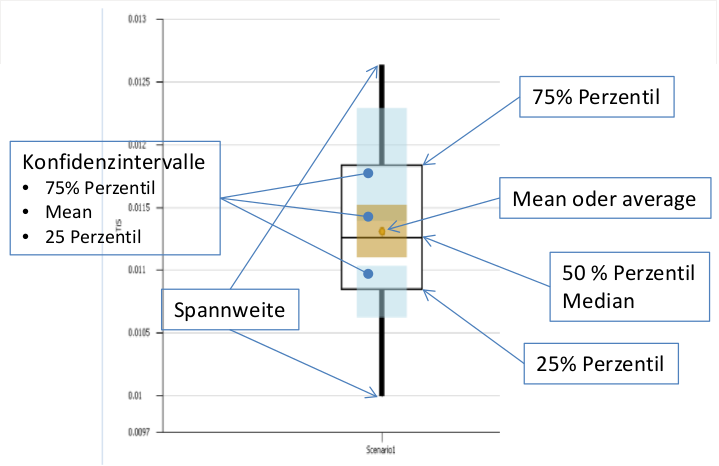
\includegraphics[scale=0.5]{images/exev_haufigkeitsverteilung_boxplot_1.png}
\caption{Boxplot Beispiel}
\label{fig:theory:boxplot:1}
\end{figure}

\subsection{Zufallsvariable}
Die Zufallsvariable lässt sich als \textit{Funktion} darstellen, die bei jedem Ergebnis eines Zufallsexperiments einen Wert (Realisierung) zuordnet. Zur Beschreibung stochastischer Phänomene sind Grössen (Variablen) zu betrachten, deren Werte vom Zufall beeinflusst werden. Beispiel eines Münzwurfs
\begin{equation}
X: \{\mbox{Wappen, Zahl}\}\rightarrow \mathbb{R},\, X(\omega) = \left\{\begin{array}{r l}1&,  \mbox{falls }\omega=\mbox{Wappen}\\-1&, \mbox{falls }\omega=\mbox{Zahl}\end{array}\right.
\end{equation}
Gegeben sei ein Wahrscheinlichkeitsaum ($\Omega, \mathcal{A}, P$).
\begin{itemize}
	\item Wahrscheinlichkeitsmass $P$ ordnet jedem Ergebnis $A \in\mathcal{A}$ seine Wahrscheinlichkeit zu:
	\begin{equation}
	P: \mathcal{A}\rightarrow [0, 1]
	\end{equation}
	\item Eine Zufallsvariable $X$ ordnet jedem Ergebniss $\omega \in \Omega$ einen Zahlenwert zu:
	\begin{equation}
	X:\Omega \rightarrow \mathbb{R}
	\end{equation}
\end{itemize}
Um die Wahrscheinlichkeit dafür zu berechnen, dass die Zufallsvariable $X$ bestimmte Werte annimmt, benötigen wir eine Verbindung zum Wahrscheinlichkeitsmass $P$ und dem System der Ereignisse.
\begin{tcolorbox}[colback=green!5,colframe=green!40!black, title=Definition der Zufallsvariable]
Eine Funktion $X: \Omega \rightarrow \mathbb{R}$, die jedem Ereignis $\omega$ eines Ergenisraums $\Omega$ eine reele Zahl $x$ zuordnet, bildet eine Zufallsvariable, falls jedes Intervall $I\in \mathbb{R}$.\\
Ist diese Teilmenge $A_i$ des Ergebnisraums $\omega$ ein \textbf{Element des Systems der Ereignisse} in einem Wahrscheinlichkeitsraum $(\omega, \mathcal{A}, P)$ so ist $P(A_i)$ die gesuchte Wahrscheinlichkeit
\end{tcolorbox}
%Beispiel Folie 7, 8
\begin{equation}\label{eq:zufallsvariable:defin}
A=\{\omega\in\Omega\vert X(\omega)\in I\}\in\mathcal{A}
\end{equation}
Das sich einstellende Ergebnis des Experiments hängt vom Zufall ab. Daher wird auch der ermittlete Zahlenwert $X(\omega)$ vom Zufall abhängen. Gesucht ist die Wahrscheinlichkeit dafür, dass $X(\omega)$ in einem bestimmten Intervall $I\subset \mathbb{R}$ liegt.\\
Zu bestimmen ist die Menge der Ergebnisse, für die $X(\omega)\in I$ gilt. Gesucht ist die Teilmenge des Ergenisraums aus \autoref{eq:zufallsvariable:defin}.
Für die Wahrscheinlichkeit des Ereignisses ${ \omega \in \Omega \vert X(\omega) \in I}$, schreiben wir abkürzend $P(X \in I)$ und entsprechend $P(a < X \leq b)$

\subsection{Theoretische Verteilungen}
%Folie 15 - 19
\subsubsection{Binominal-Verteilung}
Anwendung findet dies wenn sich beispielsweise ein Zufallsexperiment nur in zwei Ergebnissen unterscheidt, das Experiment n-mal wiederholt wird (Zufallsstichprobe vom Umfang n). Gesucht ist meist die Wahrscheinlichkeit, dass bei n-maliger Durchführung des Experimentes das Ereignis: genau, mindistens oder höchstens x-mal Eintrifft.
\begin{itemize}
	\item Wahrscheinlichkeitsfunktion: 
	\begin{equation}
	f(x)=P(X=x)={n \choose x}p^{x}(1-p)^{n-x}
	\end{equation}
	\item Erwartungswert: 
	\begin{equation}
	E(X) = n\cdot p
	\end{equation}
	\item Varianz
	\begin{equation}
	Var(X) = n\cdot p(1-p)
	\end{equation}
\end{itemize}
\subsubsection{Poisonverteilung}
Diese Verteilung wird angewendet, wenn man sich dafür interessiert, wie hoch die Wahrscheinlichkeit ist, dass das Ergebnis $E$ in einem Intervall genau oder höchstens x-mal eintritt, wenn bekannt ist, dass in diesem Intervall das Ereignis im Mittel $\mu$-mal auftritt. $\mu$ gibt eine Rate pro Zeitintervall an.
\begin{itemize}
	\item Wahrscheinlichkeitsfunktion:
	\begin{equation}
	f(x) = P(X=x) = \frac{\mu^{x}}{x!} e^{-\mu}
	\end{equation}
	$x$: Anzahl der Ereignisse z.B Ereignis $x$ tritt $1, 2, \ldots, n$-mal bei der Rate Beobachtungsintervall $\mu$ ein. 
	\item Erwartungswert/Varianz
	\begin{equation}
	E(X) = Var(X)=\mu
	\end{equation}
\end{itemize}
\subsubsection{Rechteckverteilung}
Die Rechteckverteilung eignet sich zur Beschreibung von Vorgängen, bei denen die Ergebnisse nur Zahlen eines bestimmten Intervalls $[a, b]$ sein können. Die Wahrscheinlichkeit, dass ein Ergebnis in ein bestimmtes Teilintervall fällt, wird nur durch dessen Länge bestimmt. Alle Ergebnisse eine bestimmten Intervalls [a, b] sind gleich wahrscheinlich und daher auch die Gleichverteilung im Intervall [a, b].\\
\textit{Hierzu gibt es keine Formeln}
\subsubsection{Exponentialverteilung}
Diese Verteilung wird angewendet, wenn man Beispielsweise die Zeitspanne zwischen zwei Anrufen in einer Telefonzentrale, die Dauer eines Telefongesprächs, die Lebensdauer eines Geräts (wenn Defekte durch äussere Einflüsse und nicht durch den Verschliess verursacht werden) ermitteln will.\\
Exponentialverteilung mit Parameter $\lambda > 0$
\begin{equation}
f(t) = \left\{\begin{array}{l l} \lambda e^{-\lambda t}&, \mbox{für }t\geq 0\\ 0 &, \mbox{sonst}\end{array}\right.
\end{equation}
\begin{equation}
F(x) = \left\{\begin{array}{l l} 1-e^{-\lambda x}&,\mbox{für $x\geq 0$}\\ 0 &,\mbox{für }x < 0\end{array}\right.
\end{equation}
\subsubsection{Weibull-Verteilung}
Diese Verteilung wird Angewendet um die Lebensdauer von Geräten oder Materialien mit Abnutzungserscheinungen zu beschreiben. $\alpha$ ist ein Skalierungsparameter, $\beta$ ist ein Formparameter.
\begin{equation}
f(t)=\left\{\begin{array}{r l}\alpha \cdot \beta \cdot t^{\beta-1}e^{\alpha t^{\beta}}&, \mbox{für }t \geq 0\\0 &, \mbox{sonst}\end{array}\right.
\end{equation}
\begin{equation}
F(x)=\left\{\begin{array}{r l} 1-e^{-\alpha x^{\beta}}&, \mbox{für }x\geq 0 \\ 0&, \mbox{für }x<0\end{array}\right.
\end{equation}
Interpretation des Formparameters $\beta > 0$
\begin{itemize}
	\item $\beta < 1$: Ausfallrate nimmt mit der Zeit ab (Ausfälle finden frühzeitig statt)
	\item $\beta = 1$: Ausfallrate konstant (zufällige äussere Einflüsse sind Ursache des Versagens)
	\item $\beta > 1$: Ausfallrate nimmt mit der Zeit zu (Alterungsprozesse)
\end{itemize}
Bemerkung: Der Parameterwert $\beta = 1$ führt auf die Exponentialverteilung welche somit einen Spezialfall der Weibull-Verteilung darstellt.
\subsubsection{Normalverteilung}\label{theorie:normalverteilung}
Die Normalverteilung ist die wohl wichtigste stetige Verteilung und spielt neben andrem in der schliessenden Statistik eine entscheidende Rolle. Der zentrale Grenzwertsatz besagt z.B: Dass sich eine Zufallsvariable $X$, die sich als Summe der $n$ Zufallsvariablen $X_1, X_2, \ldots, X_n$ ergibt, nähreungsweise normalverteilt ist, wenn die Anzahl der Zufalls-variablen hinreichend gross ist, die Zufallsvariablen $X_1, X_2,\ldots , X_n$ unabhängig sind oder nicht eine der Zufallsvariablen $X_1, X_2, \ldots ,X_n$ stark dominant ist (sehr salopp formuliert).
%TODO 5-Folie 36 Fehlende Formel
\begin{itemize}
	\item Wahrscheinlichkeitsdichtverteilung
	\begin{equation}
	f(x) == \frac{1}{\sigma\sqrt{2\pi}}e^{-\frac{1}{2}\left(\frac{x-\mu}{\sigma}^{2}\right)}\, , \sigma > 0
	\end{equation}
	\item Verteilungsfunktion:
	\begin{equation}
	F(x) = \int\limits_{-\infty}^{x}\frac{1}{\sigma\sqrt{2\pi}}e^{-\frac{1}{2}\left(\frac{t-\mu}{\sigma}\right)^2}\mathrm{d}t\, ,\sigma > 0
	\end{equation}
	Dieses Integral lässt sich leider nicht lösen Das bedeutet, dass wir keine Stammfunktion finden.
	\item Erwartungswert
	\begin{equation}
	E(X) = \mu
	\end{equation}
	\item Varianz
	\begin{equation}
	Var(X) = \sigma
	\end{equation}
\end{itemize}
Die Normalverteilung ist eine stetige symmetrische Verteilung. Das Maximum der Dichteverteilung liegt bei $x_{max}=\mu$. Die Wendepunkte liegen bei $x_w=\mu\pm\sigma$. Die Verteilungsfuntkon mit den Werten $\mu=0$ und $\sigma=1$ wird als Standart-Normalverteilung bezeichnet. $N(0;1)=F_0(x)$.
\begin{equation}
z=\frac{x-\mu}{\sigma}
\end{equation}
Zwischen einer Verteilungsfunktion $F(X)$ und einer Standartnormalverteilung gibt es die folgende Beziehung.
\begin{equation}
F(x)=F_0\left(\frac{x-\mu}{\sigma}\right)
\end{equation}
Daher reicht es aus, nur die Standartnormalverteilung zu kennen,diese wird in Tabellen angegeben.
%Beispiele
\subsubsection{Simulation und Zufallsvariable}
In einem dynamischen Simulationsexperiment:
\begin{itemize}
\item Werden Ereignisse (Events) zu zufälligen Zeiten erzeugt oder zerstört
\item Unterliegen Bearbeitungszeiten stochastischen Schwankungen
\item Sind Entscheidungen im Event-Flow zufällig
\item schwankungen Mengenangaben von Gütern, Nachfragen, Ressourcen etc.
\item Die Beschreibung dieser scheinbar zufälligen Prozesse erfolgt durch die Definition geeigneter Zufallsvariablen
\end{itemize}
%Definitionen der Verteilungen Folie 45
\subsection{Grundlagen der schliessenden Statistik}
%BILD Wahrscheinlichkeitstheorie
%BILD Schliessende Statistik
Die schliessende Statistik befasst sich mit Messreihen deren konkrete Ausprägung vom Zufall beeinflusst werden. Diese Messreihen können ebenfalls charakteristische Grössen etwa in Form des arithmetischen Mittels und der Varianz zugeordnet werden. Hier stellt sich die Frage nach der Gestalt des unbekannten Verteilungsgesetzes unter dem die vorliegende Realisierung zustande kam. Eine Entscheidung über die Annahme oder Ablehnung einer angenommenen Verteilung kann durch ein Vergleich der gemessenen charakteristischen Grössen der Realisierung und aus der Theorie abgeleiteten charakteristischen Grössen des hypothetischen Verteilungsgesetzes getroffen werden.
\pagebreak[2]
\subsubsection{Stichprobenerhebung}
\begin{itemize}
	\item Einfache Zufallsstichprobe
	\item Geschichtete Stichprobe
	\item Klumpenstichprobe
	\item Systematische Stichprobe
	\item Mehrstufige Stichprobe
\end{itemize}
Um gut Stichproben zu erheben muss man folgende Punkte beachten
\begin{enumerate}
\item Im Rahmen der Datenerhebung
\subitem Isolierende Abstraktion\\
Hier sind die unterschiedlichen Eigenschaften der Stichprobenerhebung zu beachten. Das passende Verfahren hängt stark von der Fragestellung und dem zu untersuchenden Objekt bzw. System ab, die durch die Simulation beantwortet werden soll. Um signifikante Aussagen machen zu können, ist die Grösse der Stichprobe zu bestimmen.
\subitem Generalisierende Abstraktion\\
Es muss eine geeignete Verteilungsfunktion gefunden werden, um die Anzahl der möglichen Experimente zu erhöhen und eine gewisse Variabilität zu ermöglichen.
\item Im Rahmen der Experimentauswertung
\subitem Festlegung der Verteilung der Eingangsdaten\\
% TODO: Überarbeiten
Sind diese festgelegt folgen die Experimente. Sind die Verteilungen zufällig, so kann diese nur durch die Festlegung eines Seeds bestimmt werden, sodass sich die Streuung um einen Mittelwert ergibt. Wurden die Eingangsdaten falsch bestimmt, wird in den folgenden Experimenten ein systematischer Fehler gemacht, der zu falschen Rückschlüssen führt
\subitem Für die Experimentplanung und Auswertung ergeben sich folgende Fragen:
\pagebreak[2]
\begin{itemize}
\item Wie sieht die Stichprobenfunktion und ihre Wahrscheinlichkeitsverteilung aus?
\item Wie kann ein Vertrauensintervall für den Mittelwert bzw. die Varianz einer Messreihe ermittelt werden?
\item Wie kann der Stichprobenumfang d.h. die Anzahl der Experimente, festgelegt werden?
\item Welche etablierten Testverfahren gibt es?
\end{itemize}
\end{enumerate}
\begin{tcolorbox}[colback=green!5,colframe=green!40!black,title=Testverteilungen]
Testverteilungen sind Verteilungen, die bei vielen statistischen Tests Verwendung finden. Wichtige Testverteilungen sind
\begin{itemize}
\item Chi-Quadrat Verteilung (\autoref{theorie:chiquadrat})
\item $t$-Verteilung (auch Student $t$-Verteilung) wenn die Stichprobe $<30$ ist (\autoref{theorie:t_verteilung})
\item Normalverteilung wenn die Stichprobe $\leq 30$ ist (\autoref{theorie:normalverteilung})
\end{itemize}
\end{tcolorbox}
%---------------------------------------------------------------------
\pagebreak[2]
\subsection{Chi-Quadrat Verteilung}\label{theorie:chiquadrat}
Dies ist eine stetige Wahrscheinlichkeitsverteilung über der Menge der positiven reellen Zahlen. Ihr einziger Parameter muss eine natürliche Zahl sein und wird Freiheitsgrad genannt. Sie ist eine der Verteilungen, die aus der Normalverteilung abgeleitet werden könne. Ha man Zufalls-variablen, die unabhängig und standardorientiert sind, so ist die Chi-Quadrat Verteilung mit Freiheitsgraden definiert als die Verteilung der Summe der quadrierten Zufalls-variablen. Solche Summen quadrierter Zufalls-variablen treten bei der Schätzung der Varianz einer Stichprobe auf.\\
Dichte der $\chi_r^2$-Verteilung mit $r$ Freiheitsgraden:
\begin{equation}\label{eq:chisqare:1}
f(t)=\left\{\begin{array}{l l} \frac{1}{2^{\frac{r}{2}}\Gamma(\frac{r}{2})}\cdot t^{\frac{r}{2}-1}\cdot e^{-\frac{t}{2}}&, \mbox{für }t > 0 \\ 0 &, \mbox{für } t \leq 0\end{array}\right.
\end{equation}
%Bild Chi Verteilung
Erwartungswert:
\begin{equation}
E(X) = r
\end{equation}
Varianz:
\begin{equation}
Var(X) = 2r
\end{equation}
%-------------------------------------------------------------------------
\subsection{Dichte der t-Verteilung}\label{theorie:t_verteilung}
Dichte der $t_r$-Verteilung mit $r$ Freiheitsgraden:
\begin{equation}
f(t)=\frac{1}{\sqrt{r}\cdot B(\frac{1}{2},\frac{r}{2})}\cdot (1+\frac{t^2}{r})^{-\frac{1}{2}(r+1)}\, , t\in\mathbb{R}
\end{equation}
Erwartungswert:
\begin{equation}
E(X) = 0 (\mbox{für }r > 1)
\end{equation}
Varianz:
\begin{equation}
Var(X) =  \frac{r}{r-2} (\mbox{für }r>2)
\end{equation}
% TODO: Bild der Verteilung
%-------------------------------------------------------------------------
Diese Verteilungen hängen von einem bzw. mehreren Parametern ab und repräsentieren somit jeweils eine ganze Klasse von Verteilungen. Sie lassen sich als Verteilungen von Zufallsvariablen definieren, die man als Funktion von standartnormalverteilten Zufallsvariablen darstellen kann. Sie lassen sich ebenfalls für hinreichend grosse Werte ihrer Parameter durch Normalverteilungen approximieren. Für den praktischen Gebrauch existieren Tabellen, deren Aufbau sich an der Anwendung in der Schliessenden Statistik orientiert. 
%-------------------------------------------------------------------------
\subsection{Konfidenzintervalle für den Wert $\mu$ der Normalverteilung}
Liegt eine konkrete Stichprobe $\{x_1,x_2,x_3,\ldots,x_n\}$ vor, so gilt für das Stichprobenmittel:
\begin{equation}
E[X] = \mu = \overline{x} = \frac{1}{n}\sum_{i=1}^n x_i
\end{equation}
Betrachtet man jeden einzelnen Wert der Stichprobe $x_i$ als zufälligen Wert der Zufallsvariablen $X_i$ so ist der Stichprobenmittelwert wieder eine Funktion, die Stichprobenfunktion: 
\begin{equation}
\overline{X}=\frac{1}{n}\sum_{i=1}^n X_i
\end{equation}
\begin{itemize}
	\item \textbf{Satz 1:} Es sei $X$ eine Zufallsvariable mit dem Erwartungswert $\mu$ und der Varianz $\sigma^2$. Fasst man den Stichprobenmittelwert als Funktion der $n$ unabhängigen Zufalls-variablen $X_i$ auf, die alle gleiche Wahrscheinlichkeitsverteilung wie $X$ unterliegen. Dann gilt
	\begin{equation}
	\overline{X}=\frac{1}{n}\sum_{i=1}^n X_i
	\end{equation}
		\subitem Der Erwartungswert
		\begin{equation}
		\overline{X} = \mu_{\overline{x}}=\frac{1}{n}\sum_{i=1}^n X_i = \mu
		\end{equation}
		\subitem Die Varianz:
		\begin{equation}
		\sigma^2_{\overline{X}}=\frac{\sigma^2}{n}
		\end{equation}
		\subitem \textbf{Interpretation: }Der Stichprobenmittelwert hat den gleichen Erwartungswert, wie die Grundgesamtheit. Dieser Mittelwert ist selbst wieder eine Zufallsvariable oder Stichprobenfunktion und streut um den Mittelwert der Grundgesamtheit. Je grösser $n$ ist, desto kleiner die Streuung oder, um so besser die Näherung.
	\item \textbf{Satz 2} Es gelten die Voraussetzungn von Satz 1. Ist $X$ darüber hinaus normalverteilt, ist auch der Stichprobenmittelwert Normal-verteilt. Ist $X$ $N(\mu;\sigma)$-verteilt, dann gilt:
	\begin{equation}
	\overline{X}\Rightarrow N(\mu ; \frac{\sigma}{\sqrt{n}})
	\end{equation}
	wobei: $\sigma$ die Standartabweichung, $\mu$ der Mittelwert und $n$ die Anzahl Stichproben ist.
\end{itemize}
\subsection{Schätzfunktion}
\subsubsection{Problembeschreibung}
Bisher sind wir davon ausgegangen, dass die Parameter $\mu$ und $\sigma$ und die Verteilungsfunktion $f$ bekannt sind.\\
Diese Annahme ist zulässig, wenn sehr viele Ergebnisse von Messungen oder Experimenten vorhanden sind. Experimente sind jedoch teuer, Zeit und Ressourcenintensiv. Es ist daher so, dass man die Anzahl der Experimente zu minimieren versucht. \textit{Mit dieser Fragestellung beschäftigt sich das DoE (Design of Experiments)}\\
Letzlich müssen die Parameter oft geschätz werden. Damit man nicht blind raten muss, werden Schätzverfahren, Schätzfunktion und Gütekriterien für die Schätzfunktion definiert.
\begin{itemize}
\item Schätzverfahren:
\subitem Haben die Aufgabe, den oder die unbekannten Parameter der Verteilung eines Merkmals in der Grundgesamtheit anhand einer Stichprobe zu schätzen.
\subitem Die Schätzung kann durch die Angabe eines einzigen Wertes erfolgen (Punktschätzung) oder durch Angabe eines Intervalls (Invervallschätzung).
\item Schätzfunktion:
\subitem Ist ein mathematischen Instrument und ordnet einer konkreten Stichprobe einen Wert zu. Sie stellt somit ein Bindeglied zwischen der Grundgesamtheit und der Stichprobe dar. Sie bildet die Beziehung zwischen den Parametern der Schätzfunktion und den entsprechenden Parametern in der Grundgesamtheit bekannt. Dabei ist die Verteilung der Schätzfunktion zumindest approximativ bekannt. So wird der Rückschluss von der Stichprobe auf die Grundgesamtheit möglich. Es erlaubt auch die Angabe des Fehlerrisikos.
\end{itemize}
\subsubsection{Gütekriterien für Schätzunktionen}
Ein Gütekriterium ist die quadratische Abweichung von Schätzfunktionen $\widehat{T}$ und Parameter $T$. Abweichung vom Schätz- oder Basiswertes $\widehat{T}$ vom Wert des Parameters der Grundgesamtheit $T$.
\begin{equation}
E[(\widehat{T}-T)^2] = Var(\widehat{T}) + [E[\widehat{T}]-T]^2
\end{equation}
$Var[\cdot]$ ist die Varianz der Schätzfunktion, $[E[\widehat{T}]-T]^2$ ist die quadrierte Abweichung von der Schätzfunktion $T$ und Parameter $T$ der Grundgesamtheit. Ist $E(\widehat{T})-T=0$ ist es Erwartungstreu.
Konstruktion dieser Funktion:
\begin{align}
\sum_{i=1}^n(x_i-\widehat{\mu})^2 \label{eq:goodcriteria:1} \\
\widehat{\mu}=\frac{1}{n}\sum_{i=1}^n x_i = \overline{x} \label{eq:goodcriteria:2}
\end{align}
Zuerst minimiert man die Summe des Schätzwertes \autoref{eq:goodcriteria:1}, danach differenziert man nach $\mu = 0$ und erhät die Schätzfunktion zu \autoref{eq:goodcriteria:2}. \\
Das Ziel des Schätzverfahrens ist, von einer Stichprobe auf eine Grundgesamtheit zu schliessen und den Fehler einer falschen Schätzung zu minimieren oder zu bestimmen.\\
Hierbei wird zwischen zwei Schätzverfahren:
\begin{itemize}
\item Punktschätzung
\subitem Für die Simulation untersuchen wir hier die Parameterschätzung für den Mittelwert $\mu$, die Varianz $\sigma^2$ und für unbekannte Wahrscheinlichkeiten $p$ (auch Anteilswerte genannt).
\nopagebreak[4]
\item Intervallschätzung
\subitem Hier geht es um die Bestimmung von Vertrauensinvervallen für die oben aufgeführten Parameter und das damit verbundene Risiko einer Fehleinschätzung oder Fehlinterpretation. Die Angabe des Fehlers oder der Genauigkeit einer Schätzung wird auch als ihre Zuverlässigkeit bezeichnet.
\end{itemize}
\begin{itemize}
	\item Mittelwert $\mu$: 
	\begin{equation}
	\overline{x} = \frac{1}{n}\displaystyle\sum^{n}_{i=1} x_i
	\end{equation}
	\item Varianz $\sigma^{2}$: 
	\begin{equation}
	s^{2}=\frac{1}{n-1} \displaystyle\sum_{i=1}^{n}(x_i - \overline{x})^{2}
	\end{equation}
	Die Varianz der Stichprobe ist abhängig von n und damit nicht Erwartungstreu. Daher wird hier die Korrektur ($n-1$) vorgenommen. Für grosse Stichproben spielt das aber keine Rolle.
	\item Anteilswert/Wahrscheinlichkeit p: 
	\begin{eqnarray}
	\overline{p} = \frac{k}{n}
	\end{eqnarray}
	 Wobei k = gute Fälle sind, und n = Stichprobenumfang
\end{itemize}

Die Verteilungsformen für das Stichprobenmittel $\overline{X}$:
\begin{table}[ht]
\ra{2}
\centering
\begin{tabular}{@{}l|ll@{}}
\toprule
Verteilung des Merkmals X & Varianz bekannt & Variant unbekannt \\ \midrule
Bekannt und normalverteilt & $\overline{X}$ ist normalverteilt & X ist t-verteilt \\ 
Bekannt und nicht normalverteilt & \multicolumn{2}{l}{\multirow{2}{*}{$X$ ist approximativ normalverteilt}} \\
Unbekannt & \multicolumn{2}{l}{} \\ \bottomrule
\end{tabular}
\end{table} \\
\subsubsection{Varianzen für die Schätzfunktion}
\begin{itemize}
\item Verteilungsformen für das Stichprobenmittel $\overline{X}$
\begin{table}[H]
\ra{2.5}
\centering
\begin{tabular}{@{}lll@{}}
\toprule
Stichprobe & Varianz $\sigma^2$ bekannt & Varianz $\sigma^2$ unbekannt \\ \midrule
Ohne Zurücklegen $\frac{n}{N}<0.05$ & $\displaystyle\sigma_{\overline{X}}^2\approx\frac{\sigma}{n}$ & $\displaystyle\widehat{\sigma}_{\overline{X}}^2\approx\frac{s^2}{n}$ \\ 
Mit zurücklegen $\frac{n}{N} \geq 0.05$ & $\displaystyle\sigma_{\overline{X}}^2=\frac{\sigma^2}{n}\cdot\frac{N-n}{N-1}$ & $\displaystyle\widehat{\sigma}_{\overline{X}}^2 =\frac{s^2}{n}\cdot\frac{N-n}{N}$ \\ \bottomrule
\end{tabular}
\end{table}
Hinweis: Das Sigma beinhaltet keinen Bruch: $\sigma_{\overline{X}}^2 \neq \sigma\frac{2}{X}$
\pagebreak[4]
\item Varianzen der Schätzfunktion $\overline{X}$
\subsubsection{Erstellen des Konfidenzintervalls}
\begin{enumerate}
	\item Feststellung der Verteilungsform von $\overline{X}$
	\item Feststellung der Varianz von $\overline{X}$ ggf. schätzen mit $s^2$
	\item Ermittlung des Quantislwertes $z$ oder $t$
	\item Berechnung des maximalen Schätzfehlers. \emph{Der maximale Schätzfehler ist das Produkt aus Quantilswert und Standartabweichung von $X$}
	\item Ermittlung der Konfidenzgrenzen \emph{Die untere und obere Konfidenzgrenze ergeben sich durch Substraktion bzw. Addition des maximalen Schätzfehlers vom bzw. zum Stichprobenmittel $X$}
\end{enumerate}
% Beispiel Folie 12
\item Die Varianzen der Schätzfunktion $P$ ergeben sich aus
\begin{equation}
P=\frac{k}{n} = \theta
\end{equation}
Für $nP(1-P) > 9$ = appriximativ normalverteilt.
\begin{table}[ht]
\ra{2}
\centering
\begin{tabular}{@{}lll@{}}
\toprule
Stichprobe & Varianz bekannt & Varianz unbekannt \\ \midrule
Mit Zurücklegen & $\sigma {2 \atop \overline{P}} = \frac{\theta(1-\theta)}{n}$ & $\widehat{\sigma}{2 \atop P} = \frac{P(1-P)}{n}$ \\
$\frac{n}{N}< 0.05$ & $\sigma {2 \atop \overline{P}} \approx \frac{\theta(1-\theta)}{n}$ & $\widehat{\sigma}{2 \atop P}\approx\frac{P(1-P)}{n}$ \\
$\frac{n}{N}\geq 0.05$ & $\sigma {2 \atop \overline{X}}=\frac{\theta(1-\theta)}{n}\cdot\frac{N-n}{N-1}$ & $\widehat{\sigma}=\frac{P(1-P)}{n}\cdot\frac{N-n}{N}$ \\ \bottomrule
\end{tabular}
\end{table}
\end{itemize}
In allen Tabellen dieses Kapitels gilt: $N$ ist die Grundmenge, $n$ die Grösse der Stichprobe und $\frac{N-n}{N-1}$ bzw. $\frac{N-n}{N}$ sind Korrekturfaktoren.\\
Erstellen eines konfidenzienintervalls
\begin{enumerate}
\item Festellung der Verteilungsform von $P$, die Schätzfunktion ist approximativ normalverteilt wenn $n P(1-P)>9$
\item Festellung der Varianz von $P$
\item Ermittlung des Quantilwertes $z$
\item Berechnung des maximalen Schätzfehlers
\subitem Der maximale Schätzfehler ist das Produkt des Quantilwerts und Standardabweichung von $P$
\item Ermittlung der Konfidenzgrenzen
\subitem Die untere und die obere Konfidenzgrenze ergeben sich durch Sustraktion bzw. Addition des maximalen Schätzfehlers vom bzw. zum Stichprobenmittel $P$
\end{enumerate}
%Beispiel Folie 15
\subsubsection{Berechnung Stichrpobenumfangs grosser Grundgesamtheiten}
Die Berechnung des notwendigen Stichprobenumfangs für die Intervallschätzung mit Zurücklegen oder Grossergrundgesamtheit unterscheidet sich vom den vorherigen Beispielen. Bisher war die Frage: Wie gross ist das Vertraunsintervall bei einer gegebenen Anzahl von Stichproben:
\begin{equation}\label{eq:stichprobenumfang:1}
-W\left(\mu - z \frac{\sigma}{\sqrt{n}}\leq \overline{x}\leq \mu + z \frac{\sigma}{\sqrt{n}}\right)=1-\alpha
\end{equation}
Jetzt soll ein maximaler Fehler vorgegeben werden
\begin{align}
\text{Fehler: }&\mu\pm e = \mu \pm z\frac{\sigma}{\sqrt{n}}\label{eq:schatzverfahren:fehler1} \\ 
\text{Wahrscheinlichkeit: }&1-\alpha\\
\text{Vorgabe: }&e\leq\pm z\frac{\sigma}{\sqrt{n}}
\end{align}
Daraus folgt bei vorgegebener Wahrscheinlichkeit $1-\alpha$ zur Bestimmung des $Z$-Wertes der Standartnormalverteilung
\begin{equation}
n \geq \frac{Z^2\sigma^2}{e^2}
\end{equation}
%Beispiel Folie 17
Bei der Berechnung des notwendigen Stichprobenumfangs für die Intervallschätzung ohne Zurücklegen, muss man anders vorgehen. Mit dem bekannten Korrekturfaktor aus \autoref{eq:schatzverfahren:fehler1}, erhält man
\begin{equation}\label{eq:schätzverfahren:2}
n \geq \frac{z^2 N \sigma^2}{e^2(N-1)+z^2\sigma^2}
\end{equation}
%Beispiel Folie 19
\subsubsection{Konfidenzinterfall für die Varianz}
Für die Schätzfunktion galt \autoref{eq:goodcriteria:1} und \autoref{eq:goodcriteria:2}, sind die $X_i$ normalverteilt gilt:
\begin{align}
s^2=\frac{\sigma^2}{n-1}\sum^n_{i=1}Z_i^2& \\
\sum_{i=1}^n Z_i^2& = \frac{s^2(n-1)}{\sigma^2}
\end{align}
Zur berechnung eines asymmetrischen Konfidenzintervall, beispielsweise durch die Chi-Quadrat Verteilung, in \autoref{eq:chisqare:1} angegeben. Das heisst die Zufallsvariable $Y$ in der die zu schäzende Varianz der Grundgesamtheit einfliesst, ist Chi-Quadrat-verteilt mit $r=n-1$ Freiheitsgraden.
\begin{align}
W\left(y_{\frac{\alpha}{2}} \leq \frac{(n-1)s^2}{\sigma^2} \leq y_{1-\frac{\alpha}{2}}\right)\\
W\left(\frac{(n-1)s^2}{y_{1-\frac{\alpha}{2}}} \leq\sigma^2 \leq\frac{(n-1)s^2}{y_{\frac{\alpha}{2}}}\right)
\end{align}
Anmerkung zu diesen Funktionen:
\begin{itemize}
\item Anstatt $r$ wird für den Freiheitsgrad oft auch $k$ verwendet
\item Die $y$-Werte (Quantilswerte für $\frac{\alpha}{2}$ bzw. $1-\frac{\alpha}{2}$ bei $r$ Freiheitsgraden) sind der Tabelle der Chi-Quadrat Verteilung zu entnehmen
\end{itemize}
%Beispiel Folie 22

\subsection{Testverfahren}
\begin{tcolorbox}[colback=green!5,colframe=green!40!black, title=Definition Testverfahren]
Im Testverfahren erhält man mit einer vorgegebenen Wahrscheinlichkeit von mindestens $1-\alpha$ auf Grund einer Stichprobe ein Intervall $[a,b]$, das einen unbekannten Parameter $v$ enthält, so heisst dieses Intervall für $v$ bei einem Vertrauensniveau von $1-\alpha$
\end{tcolorbox}
$\alpha$ wird in diesem Zusammenhang auch als Signifikanzzahl bezeichnet und ist ein Mass für die Irrtumswahrscheinlichkeit. Das heisst die Null-Hypothese abzulehnen, obwohl sie richtig ist. Damit hat man auch eine Aussage über die Wahrscheinlichkeit eines Fehlers.
\pagebreak[4]
\subsubsection{Fehler erster Art}
Der Fehler ersten Art, bedeutet fehlerhaftes Ablehnen einer Hypothese. Liegt der ermittelte Wert ausserhalb des Annahmebereichs, so wird die Hypothese verworfen. Die Wahrscheinlichkeit, dass die Hyptohese fälschlicherweise verworfen wird, wird durch die Fläche unter der Verteilungsfunktion ausserhalb des Annahmebereichs repräsentiert und lässt sich bestimmen als $\alpha$.
\begin{figure}[H]
\centering
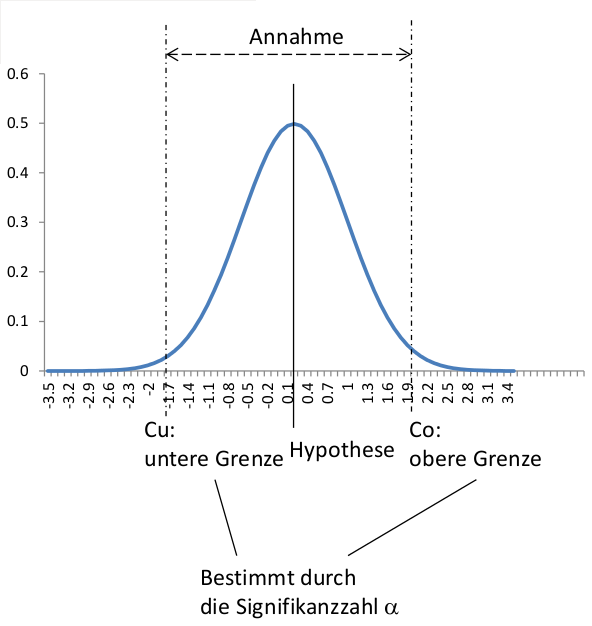
\includegraphics[scale=0.25]{images/exev_testverfahren_fehlerart_1.png}
\caption{Fehler ersten Art}
\label{fig:testverfahren:fehler1}
\end{figure}
\subsubsection{Fehler zweiter Art}
Der Fehler der zweiten Art, bedeutet eine fehlerhaftes Annehmen einer Hypothese. 
\begin{figure}[htb]
\centering
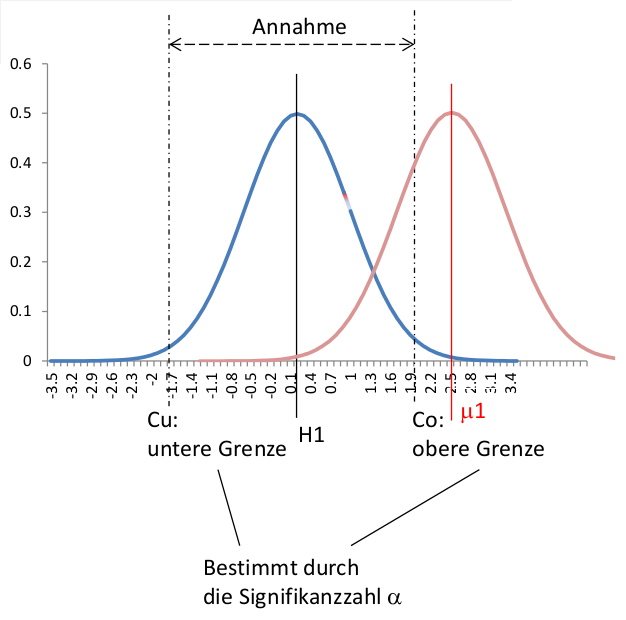
\includegraphics[scale=0.25]{images/exev_testverfahren_fehlerart_2.png}
\caption{Fehler zweiter Art}
\label{fig:testverfahren:fehler2}
\end{figure}
Beim Aufstellen einer Hypothese kann es passieren, dass diese nicht komplett der Wahrheit entspricht. Der Fehler der Hypothese und der Wahrheit wird als Fehler $\beta$ durch die Fläche von $\infty$ bis an das Ende der Annahme angegeben.
\subsubsection{Fallunterscheidungen}
Man kann unter verschiedenen Fällen unterscheiden. Unter anderem:
\begin{itemize}
\item Der/die interessierenden Parameter der Grundgesamtheit sind z.B als Erfahrungswert bekannt. Durch Stichproben soll überprüft werden, ob diese Werte noch eingehalten werden. 
\item Hypothesen basieren auf Sollwerten und Normen. Diese Werte müssen also durch Vorgaben eingehalten werden. es ist zu überprüfen, ob ein Standard eingehalten wird.
\item Hypothesen aufgrund einer Theorie oder auch auf Grund von Ergebnissen aus Simulationsläufen.
\end{itemize}
Ein statistischer Test ist eine Methoden, die eine Entscheidung ermöglichen soll. Deshalb braucht man ein bestimmtes Verfahren, um Hypothesen zu testen.
\begin{enumerate}
\item Festlegen der Grundgesamtheit und Formulieren der Nullhypothese $H_0$ und der Alternativhypothese $H_1$ (im Allgemeinen die Verneinung der Nullhypothese)
\item Festlegen der Signifikanzzahl $\alpha$, gibt die Irrtumswahrscheinlichkeit an oder das Vertrauensintervall $1-\alpha$
\item Bestimmen der Testgrösse und des Annahme und Ablehnungsbereichs. Testgrösse kann der Stichprobenmittelwert sein
\item Berechnen des Wertes der Testgrösse mit den Daten der Stichprobe und Testentscheidung
\end{enumerate}
Um Hypothesen zu beweisen, formuliert man oft eine Verneinung dieser Hypothese als Nullhypothese und versucht dann, diese durch einen statistischen Test zu wiederlegen. Dies ist Vergleichbar mit dem Indirekten Beweis der Mathematik.
\subsubsection{Parametertest}
Der Paramtertest überprüft die Hypothese über Paramter einer Grundgesamtheit.
\begin{equation}
\mu_{0} - z \frac{\sigma}{\sqrt{n}}\leq\overline{x}\leq\mu_{0}+z \frac{\sigma}{\sqrt{n}} \label{eq:parameter:1}
\end{equation}
Die Fragen die sich beim Paramtertest stellen sollten sind:
\begin{itemize}
\item Liegt eine systembedingte Störung vor?
\item Ist der angegebene Mittelwert korrekt?
\item Liegt das Ergebniss im Bereich der statistischen Schwankungsbreite (Tolleranz)?
\end{itemize}
Diese Fragen können über das Vertrauensintervall (\autoref{eq:parameter:1}) beantwortet werden.
%BEISPIEL: Folie 11
\subsubsection{Anteilswerte}
Diese können analog zu den Paramtertests angewendet werden:
\begin{enumerate}
\item Wähle die Signifikanzzahl $\alpha$ und bestimme daraus die Werte für $Z$ aus der Tabelle ($1-\alpha$)
\item Berechne die Annahmegrenzen 
\end{enumerate}
\begin{align}
c_u &= p_0 - z\displaystyle\sqrt{\frac{p_0(1-p_0)}{n}}&\quad\mbox{oder} \\
c_u &= p_0 - z\displaystyle\sqrt{\frac{p_0(1-p_0}{n}}\,\sqrt{\frac{N-n}{N-1}}&\quad\mbox{und} \\
c_0&=p_0 + z\displaystyle\sqrt{\frac{p_0(1-p_0)}{n}}&\quad\mbox{oder} \\
c_0&= p_0 + z \displaystyle\sqrt{\frac{p_0(1-p_0)}{n}}\,\sqrt{\frac{N-n}{N-1}}&
\end{align}
\begin{enumerate}
  \setcounter{enumi}{2}
  \item Man berechne den Anteil $\overline{p}=\frac{k}{n}$
  \item Fällt $\overline{p}$ in den Annahmebereich: $c_u\leq\overline{p}\leq c_0$, wird die Hypothese angenommen, sonst abgelehnt.
\end{enumerate}
%BEISPIEL Folie 15
\subsubsection{Differenztests}
Manchmal will man mit Hilfe von Stichproben untersuchen, ob  zwei Mittelwerte $\mu_1 = \mu_2$ sind, oder signifikant voneinander abweichen. Zum Beispiel ist das Ergebnis des einen (Simulations)Experiments signifikant unterschiedlich von dem anderen.  Dabei werden zwischen zwei Stichproben unterschieden
\begin{itemize}
\item Abhängige Stichproben
\subitem Diese werden in der Regel angestrebt, wenn es sonst zu Überlagerungen kommt, die das Ergebnis verzerren könnten.
\item Unabhängige Stichproben
\subitem Diese liegen dann vor, wenn zum Beispiel für ein Herstellungsprozess zwei unterschiedliche Modellvarianten untersucht werden sollen, in denen der Durchsatz untersucht werden soll.
\end{itemize}
Abhängige Stichproben erstellen:
\begin{enumerate}
\item Bilden der Nullhypothese
\begin{equation}\label{eq:differenz:nullhyp}
H_0: \mu_1 = \mu_2
\end{equation}
\item Die Differnezen der Stichprobe müssen für alle $i$ erfasst werden
\begin{equation}\label{eq:differenz:diff}
d_i = x_i - y_i
\end{equation}
\item Dann gilt die Nullhypothese $H_0$ gleich, wenn der Mittelwert von $d_i$ im Bereich von $1-\alpha$ liegt
\item Es wird die Signifikanzzahl $\alpha$ gewählt
\item Mit Hilfe der Tabelle für Normalverteilung werden die Annahmegrenzen festgelegt
\end{enumerate}
Unabhängige Stichproben erstellen:
\begin{enumerate}
\item Lege eine Signifikanzzahl $\alpha$ fest
\item Mit Hilfe der Tabelle für Normalverteilung wird der Werte $\mp Z$ festgelegt
\item Berechnung des Annahmebereichs
\footnote{Nach wie vor ist der Mittelwert gleich dem Mittelwert der Differenz. Aber jetzt muss die Varianz für jede Probe separat angenommen bzw. Geschätz werden.}
\begin{equation}
c=\mp z\sqrt{\frac{\sigma_1^2}{n_1}+\frac{\sigma_2^2}{n_2}}
\end{equation}

\item Berechnung der Mittelwerte der Stichproben $\mu_1$ und $\mu_2$
\item Man nehme die Nullhypothese aus \autoref{eq:differenz:nullhyp} an, wenn die Differenz aus \autoref{eq:differenz:diff} in den Annahmebereich fällt
\end{enumerate}
%BEISPIELE
\subsubsection{Verteilungstests}
Bisher wurden Tests behandelt, die sich auf Parameter der Grundgesamtheit beziehen. Nun soll mithilfe von Stichproben überprüft werden, ob Hypothesen über Wahrscheinlichkeitsverteilungen überprüft werden können. Verbreitete Testverfahren in den Verteilungstests sind:\footnote{Als einziger dieser Verfahren haben wir die Chi-Quadrat Verteilung behandelt}
\begin{itemize}
\item Chi-Quadrat Test (\autoref{theorie:chiquadrat})
\item Kolmogoroff-Smirnoff Test
\item Spezielle Tests, die für die Überprüfung bestimmter Verteilungen zugeschnitten sind
\end{itemize}
Die Idee des $\chi$-Quadrat Test ist, es werden die Häufigkeiten der empirische ermittelten Verteilun mit der theoretischen Verteilung verglichen. Dazu werden wieder die Differenzen der Häufigkeitswerte quadriert, normiert und aufaddiert.
\begin{align}\label{eq:testverfahren:verteilung1}
y=&\sum_i^m \frac{\left(n_i - np_i\right)^2}{np_i}\\
y=&\sum_i^m \frac{\left(h_i^e-h_i^{th}\right)^2}{h_i^{th}}
\end{align}
Geht man davon aus, dass die einzelnen Messungen wieder Normalverteilt sind, dann ist die Summe $y$ Chi-Quadrat verteilt mit $m-1$ Freiheitsgraden.\\
Um den Test zu erhalten, geht man folgendermassen vor:
\begin{enumerate}
%\setcounter{enumi}{0}
\item $H_0$: Die empirische Häufigkeit entspricht der theoretischen Häufigkeit
\item Man wähle eine Signifikanzzahl $\alpha$ und bestimme die Anzahl der Freiheitsgrade
\subitem Sind alle Parameter der Verteilungfunktion bekannt, haben wir $m-1$ Freiheitsgrade
\subitem Wenn die Parameter der Verteilungsfunktion geschätzt werden müssen, kann die Anzahl Freiheitsgrade für jeden geschätzen Parameter um eins reduziert werden.
\item Die Annahmegrenze $C_o$ wird aus der Tablle für die Chi-Quadrat Verteilung ermittelt. Die Häufigkeit sollte nicht kleiner als 5 und der Stichprobenumfang nicht grösser als 30 sein. Sonst muss man mit der YATES Korrektur arbeiten
\item Man berechnet für die vorliegenden Sithcproben den Testwert mit \autoref{eq:testverfahren:verteilung1}
\item Gilt $Y>C_0$, dann lehnt man die Hypothese $H_0$ ab, ansonsten nimmt man sie an
\end{enumerate}
%BILD folie 26
\subsubsection{Unabhängigkeitstest}
Die Unabhängigkeitstests beinhaltet die Überprüfung von eventuellen Abhängigkeiten zwischen bestimmten Zufallsvariablen. Man spricht auch von einem Chi-Quadrat Unabhängigkeitstest. Voraussetzungen dafür sind, dass die Häufigkeit grösser als 5 ist und der Stichprobenumfang grösser als 30. Dieser Test liefert eine Entscheidung ob eine Abhängigkeit besteht, jedoch keine Information oder Mass über die Stärke der Abhängigkeit (siehe \autoref{theorie:regression}). Sind diese Voraussetzungen nicht erfüllt können Korrekturen vorgenommen werden, die sogenannte YATES Korrektur. Da es jedoch auch hier keine festen Regeln gibt, und die Ergebnisse mit Vorsicht zu bewerten sind, sollten aus praktischer Sicht die Voraussetzungen erfüllt werden.
%BEISPIEL
\subsection{Zusammenhang zwischen zwei Merkmalen}
Dem Erkennen des Zusammenhangs zwischen zwei oder meBhr Merkmalen kommt der betrieblichen Praxis eine grosse Bedeutung zu. Bei der Untersuchung des Zusammenhangs zwischen zwei Merkmalen X und Y sind folgende Fragen interessant:
\begin{itemize}
\item Besteht ein Zusammenhang zwischen X und Y? (siehe \autoref{theorie:chiquadrat})
\item Von welcher Form ist der Zusammenhang?
\item Von welcher Stärke (Intensität) ist der Zusammenhang?
\end{itemize}
\begin{tcolorbox}[colback=green!5,colframe=green!40!black, title=Abhängigkeit]
Zwei Merkmale sind statistisch unabhängig, wenn der Wert des einen Merkmals nicht davon abhängt, welcher Wert das andere Merkmal besitzt. Sonst sind sie abhängig.
\end{tcolorbox}
Zu unterscheiden sind dabei:
\begin{itemize}
\item Formale Abhängigkeit: 
\subitem Liegt eine zahlenmässig begründete Abhängigkeit zwischen den Merkmalen vor?
\item Sachliche Abhängigket?
\subitem Ist der Wert des einene Merkmals ursächlich für den Wert des anderen Merkmals? Die Feststellung der Kausalität bzw. der Ursache-Wirkungsbeziehung kann die Zusammenarbeit mit dem auf dem jeweiligen Sektor Fachkundigen erforderlich machen. Hier muss man sich aber vor "Unsinns-Korrelationen" in acht nehmen.
%BEISPIEL Folie 5 -7
\end{itemize}
Herausfinden ob eine Tabelle unabhängig ist
\begin{equation}\label{eq:zusammenhang:1}
h_{i,k}=\frac{h_i h_{i,k}}{n}
\end{equation}
%%%%%%%%%%%%%%%%%%%%%%%%%%%%%%%%%%%%%%%%%%%%%%%%%%%%%%%%%%%%%%%%%%%%%%
\subsubsection{Regressionsanalyse}\label{theorie:regression}
Die Regressionsanalyse beschreibt die Form bzw. Tendenz des Zusammenhangs durch eine mathematische Funktion. Durch sie werden die Wertkombinationen $(x,y)$ der Merkmalsträger in ein Koordinatensystem eingetragen, dann ergitb sich ein sogenanntes Streuungsdiagramm (Punktewolke). In der linearen Regressionsanalyse wird die Tendenz durch die Funktion bestimmt.\\
%BILD Folien 8,9
\begin{itemize}
\item Bei einseitiger Beeinflussung (y wird nur durch den Parameter x bestimmt)
\begin{equation}
y=a_1+b_1\cdot \label{eq:depency:1}
\end{equation}
\item Bei wechselseitiger oder unbekannter Abhängigkeit zusätzlich \footnote{Achtung, dies ist keine Umkehrfunktion von \autoref{eq:depency:1}}
\begin{equation}
x=a_2+b_2\cdot y
\end{equation}
\end{itemize}
Dabei müssen jedoch die Parameter $a$ und $b$ bekannt sein. Zur bestimmung dieser verwendet man kleine Quadrate. Die Aufgabe besteht darin, \autoref{eq:regression:1} zu minimieren. Dies erreicht man mit partiellem Ableiten des Ausdrucks nach $a$ und $b$, nullsetzen der beiden partiellen Ableitungen und auflösen der beiden Gleichungen nach $a$ und $b$. 
\begin{equation}\label{eq:regression:1}
\sum_i^n \left(y_i - a - bx_i\right)^2
\end{equation}
Dies ergibt:
\begin{align}
a_1 =& \overline{y} + b_1\overline{x} \label{eq:regression:4-1}\\
b_1 =& \frac{\sum_{i=1}^n x_i y_i - n\overline{x}\overline{y}}{\sum_{i=1}x_i^2-n\overline{x}^2} \label{eq:regression:4-2}
\end{align}
Analog folgt für:
\begin{align}
x=a_2+b_2y &\Longleftrightarrow& a_2=\overline{x}+b_2\overline{y}\\
&\Longleftrightarrow& b_2 = \frac{\sum_{i=1}^n x_i y_i - n\overline{x}\overline{y}}{\sum_{i=1}y_i^2-n\overline{y}^2}
\end{align}
%BEISPIEL Folie 10,11
%%%%%%%%%%%%%%%%%%%%%%%%%%%%%%%%%%%%%%%%%%%%%%%%%%%%%%%%%%%%%%%%%%
\subsubsection{Korrelation}
Die Korrelationsanalyse hat die Aufgabe:
\begin{itemize}
\item Die Stärke (Intensität) des Zusammenhangs festzustellen
\item Wie ausgeprägt der Einfluss des einen Merkmals auf das andere Merkmal ist
\item Zur Bewertung dieses Einflusses sind Kenngrössen zu entwickeln bzw. zu berechnen
\end{itemize}
Je nach Skalierungsgrad stehen verschiedene Verfahren zur Verfügung:
\begin{enumerate}
\item Sind beide Merkmale mindestens Intervallskaliert:
\subitem Korrelationskoeffizienz von Bravais Pearson
\item Ist ein Merkmal ordinalskaliert und das ander Merkmal mindestens ordinalskaliert:
\subitem Rangkorrelationskoeffizient von Spearman
\item Ist mindestens eines der beiden Merkmale Nominalskaliert:
\subitem Kontingenzkoeffizienten und Assoziationsmasse
\item Grundsätzlich können Skalierungsvoraussetzungen von den Merkmalen überfüllt sein, dies ist jedoch nicht ratsam, da das mit einem Informationsverlust verbunden ist.
\end{enumerate}
\subsubsection{Bravais Pearson}
\begin{enumerate}[label=\bfseries \arabic*. Schritt: ]
\item Kovarianz\\
Diese ist ein Mass für die Streuung der Merkmalsträger bzw. deren Merkmalswertkombinationen $(x_i, y_i)$ um den Mittelpunkt oder Durchschnitt $(\overline{x}, \overline{y})$. Die Kovarianz erfolgt analog zu der, der Varianz
%BILD
Formel:
\begin{align}
\sigma_{XY}&=&\frac{1}{n}\sum_{i=1}^n (x_i-\overline{x})(y_i-\overline{y})\label{eq:regression:2}\\
\sigma_{XY}&=&\frac{1}{n}\sum_{i=1}^n x_i y_i - \overline{xy}\label{eq:regression:3}
\end{align}
\item Normierung der Kovarianz\\
Es entsteht der Korrelazionskoeffizient (Normiert wird auf den Wertebereich $[-1,1]$
\begin{equation}
r=\frac{\sigma_{XY}}{\sigma_X\sigma_Y}
\end{equation}
oder etwas ausführlicher
\begin{equation}
r=\frac{\sum_{i=1}^n(x_i-\overline{x})(y_i-\overline{y})}{\sqrt{(\sum_{i=1}^n(x_i-\overline{x})^2)(\sum_{i=1}^n (y_i-\overline{y})^2)}}
\end{equation}
Durch Umformung gilt
\begin{equation}
r=\sqrt{b_1 b_2}
\end{equation}
Dabei ist $r$ positiv zu setzen, wenn beide Steigungsmasse positiv sind, oder negativ wenn beide Steigungsmasse negativ sind. Dazu benötigen wir aber \autoref{eq:regression:2} und \autoref{eq:regression:3}
\end{enumerate}
\subsubsection{Interpretation des Korrelationskoeffizienten von Bravais Pearson}
Der Korrelationskoeffizient r berechnet sich zu $r$.
\begin{align}
r&=\frac{\sigma XY}{\sigma X \sigma Y} =& \frac{\sum_{i=1}^n\left(x_i-\overline{x} \right )\left(y_i - \overline{y} \right )}{\sqrt{\left(\sum_i^n\left(x_i - \overline{x}\right)^2 \right )\left(\sum_i^n\left(y_i - \overline{y} \right )^2 \right )}}\\
b_1 &=& \frac{\sum_{i=1}^n x_i y_i - n\overline{x}\overline{y}}{\sum_{i=1}^n x_i^2 - n\overline{x}^2}&\\
b_2 &=& \frac{\sum_{i=1}^n x_i y_i - n\overline{x}\overline{y}}{\sum_{i=1}^n y_i^2 - n\overline{y}^2}&
\end{align}
\begin{itemize}
\item bei positivem $r$ ist der lineare Zusammehang der Merkmale $X$ und $Y$ positiv, bzw gleichläufig
\item bei negativem $r$ ist der lineare Zusammehnahng der Merkmale $X$ und $Y$ negaziv bzw. gegenläufig
\item Der Betrag von $r$ kann die Werte 0 bis 1 annehmen. 1 bedeutet sehr startker linearer Zusammehnang, 0 kein linearer Zusammehnang. Die beiden Regressionsgeraden stehen senkrecht aufeinander
\end{itemize}
%%%%%%%%%%%%%%%%%%%%%%%%%%%%%%%%%%%%%%%%%%%%%%%%%%%%%%%%%%%%%%%%%%%%%
\subsubsection{Zeitreihe}
\begin{tcolorbox}[colback=green!5,colframe=green!40!black, title=Zeitreihe]
Eine Zeitreihe ist eine zeitlich geordnete Folge von Merkmalswerten. 
\begin{itemize}
\item Kosten/Gewinnentwicklung
\item Verbrauch von Ressourcen
\item Auftrangseingang
\item Bearbeitungs oder Durchlaufzeiten
\end{itemize}
Die Aufgabe der Zeitreihenanalyse besteht darin, eine Struktur und Gesetzmässigkeit einer Zeitreihe zu erkennen. Sie ist ein Mittel zur Progrnose, oder erkennen eines Trends.
\end{tcolorbox}
Der Trend beschreibt die langfristige Grundrichtung einer Zeitreihe. Um ihn streuen die Zeitreihenwerte im Zeitablauf unf für seine Entwicklung sind dauerhaft wirksame Einflüsse verantwortlich. Der Verlauf kann linear oder nichtlinear sein. Wenn er nichtlinear ist, kann er sich einer Exponential, Potenz oder Logistische Funktion annhähern. Die nichtlinearen Verläufe entziehen sich häufig aber der intiuitiven Vorstellung werden daher oft falsch bewertet.
Die Zeitreihe hat aber einige Stolpersteine. Beispielsweise ist es nicht immer einfach periodische Schwankungen zu erkennen oder besonderer Ereignisse zu identifizieren. Lösen lasen sich diese Probleme durch sogenanntes Glätten des Verlaufs durch beispielsweise den gleitenden Durchschnitt oder die Methode der kleinsten Quadrate (siehe Regression:\autoref{theorie:regression}).
\newpage
\section{Beispiele}
%TODO: Beispiel hinzufügen, mit Formel verknüpfen
\subsection{Mittelwerte und Spannweite}\label{praxis:mittelwerte}
\begin{table}[h]
\ra{1.2}
\centering
\begin{tabular}{@{}lllllll@{}}
\toprule
Versicherungssumme\\ in Tsd & Anzahl Verträge & Median der Klasse & $x_ih_i$ & $H_j$ & Std. Abweichung & Varianz \\ \midrule
4-10 & 20 & 7 & 140 & 20 & 481 & 11568.05 \\
10-20 & 160 & 15 & 2400 & 180 & 2568 & 41214.4 \\
20-30 & 80 & 25 & 2000 & 260 & 484 & 2928.20 \\
30-40 & 40 & 35 & 1500 & 300 & 158 & 624.1 \\
40-80 & 88 & 50 & 5280 & 388 & 2547.6 & 73752.02 \\
80-120 & 12 & 100 & 1200 & 400 & 827.4 & 57049.23 \\ \bottomrule
\end{tabular}
\end{table}
\begin{itemize}
\item Durchschnittliche Versicherungssume(\autoref{theorie:mittelwerte:arith}):
\begin{equation*}
\overline{x} = \frac{1}{n}\sum_j x_jh_j = \frac{1}{400}\cdot 12420=3105
\end{equation*}
\item Dichte (\autoref{theorie:mittelwerte:dicht})
\begin{align*}
d_1=\frac{20}{10-4}=3.33, d_2=16, d_3=8, d_4=4, d_5=2.2, d_6=0.3
\end{align*}
\item Modus\\
Aus den Dichten lässt sich herauslesen, dass Klasse 2 die höchste Dichte hat, diese ist also die Modusklasse. Berechnung des Modus(\autoref{theorie:mittelwerte:modus:2})
\begin{equation*}
\ra{2}
\begin{array}{rcccl}
M_0 &=& x_2^u+\displaystyle\frac{d_2-d_1}{(d_1-d_1)+(d_2-d_3)}\cdot(x_2^o-x_2^u)&& \\
M_0 &=& 10+\displaystyle\frac{16-3.33}{(16-3.33)+(16-8)}\cdot(20-10) &=& 16130
\end{array}
\end{equation*}
\item Median\\
Der Median ist der Wert der geordneten Mitte von 400 (Summe aller Verträge), also 200. Diese Anzahl kommt in der 3. Klasse zu liegen. Damit ergibt sich der Median(\autoref{theorie:mittelwerte:quant}):
\begin{equation*}
\ra{2}
\begin{array}{rcccl}
M_e&=&x_3^u+\displaystyle\frac{\frac{n}{2}-H_2}{h_3}(x_3^o-x_3^u)&&\\
M_e&=&20+\displaystyle\frac{400\div2-180}{80}(30-20)&=&22500
\end{array}
\end{equation*}
\item Quantil\\
Die erste Quantilklasse it $\frac{400}{4}=100$. Dies ist in Klasse 2. Analog zum Median berechnet sich das erste Quantil(\autoref{theorie:mittelwerte:quant}).
\begin{equation*}
\begin{array}{rcccl}
Q_1&=&x_2^u+\displaystyle\frac{\frac{n}{4}-H_1}{h_2}(x_2^o-x_2^U)&&\\
Q_1&=&10\displaystyle\frac{400\div4-20}{160}(20-10)&=&50000
\end{array}
\end{equation*}
Das zweite Quantil ist der Median und das dritte Quantil entspricht dem ersten Quantil plus dem Median. 
\pagebreak
\item Quantils und Dezilabstände\\
\subitem Quantilsabstände: Der Quantilsabstand bewegt sich 50\% um den Median.
\begin{equation*}
\begin{array}{rcl}
Q_3-Q_1&=&ZQA\\
40000 - 15000&=&25000
\end{array}
\end{equation*}
\subitem Dezilabstände\\
\begin{equation*}
\begin{array}{rcccl}
D_j&=&x_j^u+\displaystyle\frac{n\cdot\frac{1}{10}-H_{j-1}}{h_j}\cdot(x_j^o - x_j^u)&&\\
D_9&=&40+\displaystyle\frac{400\cdot\frac{9}{10}-300}{88}\cdot(80-40)&=&67270
\end{array}
\end{equation*}
Der Dezilabstand ist $D_9-D_1=56020$.
\end{itemize}
%------------------------------------------------------------------------------------------
\subsection{Grundlagen der schliessenden Statistik}
\begin{enumerate}
\item Es sei X die Zufallsvariable X = Augenzahl bei Würfeln, dann galt für einen Wurf: $\mu=3.5, \sigma^2=2,92$. Wie sieht die Häufigkeit (Wahrscheinlichkeit), Varianz, Mittelwerte bei einem, zwei oder drei Würfen aus?\\
% TODO: Tabelle schreiben
Die 5 tritt 4 mal auf, die 6 Tritt 10 mal auf.
\begin{table}[ht]
\centering
\begin{tabular}{@{}llll@{}}
\toprule
 & 1. Wurf & 2. Wurf & 3. Wurf \\ \midrule
Mittelwert $\mu$ & 3.5 & 3.5 & 3.5 \\
Varianz$\sigma^2$ & 2.92 & $\frac{2.92}{2}=1.46$ & $\frac{2.92}{3}=0.97$ \\
Std. Abweichung $\sigma$ & 1.71 & 1.21 & 0.98 \\ \bottomrule
\end{tabular}
\end{table}
% TODO: Bilder der Würfe
\item Sie haben ein Situationsmodell einer Produktionseinrichtung erstellt, vom realen System wissen sie, dass diese Maschine im normalverteilten Mittel 10 Stück pro Sekunde produziert und die Standardabweichung von 1 Stück pro Sekunde besitzt. Sie führen der Simulationsumgebung 25 Experimente (Replications) durch. 
\subitem Mit welcher Wahrscheinlichkeit wird der mittlere Ausstoss zwischen 9.8 und 10.2 Stück pro Sekunde liegen?
\subitem Mit welcher Wahrscheinlichkeit wird der Ausstoss über 10.2 liegen?
\subitem Wie verändert sich das Ergebniss, wenn sie statt dessen nur 5 bzw. 100 Experimente machen?\\
Mit $\mu = \frac{10 S}{sec}$ und $\sigma=\frac{1 S}{sec}$. Daraus folgt:
\begin{equation*}
Z_{\mbox{Stichprobe}}=\frac{\overline{X}-\mu}{\frac{\sigma}{\sqrt{n}}}
\end{equation*}
Gesucht ist nun:
\begin{equation*}
\ra{2}
\begin{array}{rcl}
&P&(9.8\geq\overline{x}\geq10.2)\\
&P&\left(\displaystyle\frac{9.8-\mu}{\frac{\sigma}{\sqrt{n}}}\geq\displaystyle\frac{\overline{x}-\mu}{\frac{\sigma}{\sqrt{n}}}\geq\displaystyle\frac{10.2-\mu}{\frac{\sigma}{\sqrt{n}}}\right)\\
\Longrightarrow&P&\left(\displaystyle\frac{9.8-10}{0.2}\geq\displaystyle\frac{\overline{x}-10}{0.2}\geq\displaystyle\frac{10.2-10}{0.1}\right)\\
&P&(Z_1\geq\overline{Z}\geq Z_2)=1-\alpha
\end{array}
\end{equation*}
\pagebreak[4]
\item In welchem symmetrischen Intervall liegt der Mittelwert bei vorgegebener Wahrscheinlichkeit, oft mit $1-\alpha$ bezeichnet. Hier sei $1-\alpha=0.9$. 
\subitem Z ist nach Voraussetzung N(0,1) verteilt, dann folgt unmittelbar: $P(-z\leq\overline{z}\leq z)=1-\alpha \Rightarrow 1-\alpha = F_0(z)-F_0(-z)$, wobei z die obere und untere Schranke bildet: 
\begin{table}[ht]
\centering
\begin{tabular}{@{}llll@{}}
\toprule
$n$ & $\sigma\div n^2$ & $Z\cdot \sigma \div n^2$ & Intervall \\ \midrule
5 & 0.45 & 0.738 & [9.262;10.738] \\
25 & 0.2 & 0.328 & [9.672;10.328] \\
100 & 0.1 & 0.164 & [9.836;10.164] \\ \bottomrule
\end{tabular}
\end{table}
Dies finden wir wiederum mit der folgenden Formel heraus:
\begin{equation*}
\overline{Z}=\frac{\overline{X}-\mu}{\frac{\sigma}{\sqrt{n}}}
\end{equation*}
Daraus folgt \autoref{eq:stichprobenumfang:1}.
\end{enumerate}
%------------------------------------------------------------------------------------------
\subsection{Schätzverfahren}
\paragraph{Beispiel} In einer Wurstfabrik werden u.a. Leberwürste hergestellt. Aus langjährigen Messreihen ist bekannt, dass das Füllgewicht der Leberwürste normalvertwilt ist. Das Soll-Mindestgewicht der Würste beträgt 125g. Aus der Tagesproduktion von 600 Würsten wurder 26 Würste zufällig ohne Zrücklegen entnommen und gewogen. Die Messergebnisse für das Füllgewicht (in Gramm) wurden in eine Tabelle eingetragen.
\begin{table}[ht]
\centering
\begin{tabular}{@{}lllllll@{}}
\toprule
128.4 & 123.8 & 123.5 & 126.9 & 125.5 & 123.1 & 124.9 \\
123.1 & 126.6 & 121.9 & 125.3 & 123.4 & 122.1 & 124   \\
123.3 & 123.2 & 123.2 & 124   & 122.8 & 127.1 & 125.7 \\
127.1 & 125.8 & 123.7 & 125.9 & 124.9 &       &       \\ \bottomrule
\end{tabular}
\end{table}\\
Die Daten haben den Mittelwert: $ \overline{X}=124.5\text{g}$ und eine Varianz $s=1.72\text{g}$.
\subparagraph{Erstellen des 95\% Konfidenzintervall:} $\mu = 26$. Da $s = \sigma^2$:
\begin{align*}
z = \frac{\sqrt{1.72}}{\sqrt{26}} = 0.2572 \\
\end{align*}
Nun muss man den gesuchrten Wert in der Tabelle der Normalverteilung nachschlagen, in unserem Fall 0.975 (weil es das Mittel von 95\% ist, und die Verteilung Normalverteilt ist, können wir einfach die hälfte von 5 dazuzählen). Dabei erhalten wir 1.96. Damit nun das Intervall festgelegt werden kann, muss man erst z mit dem Wert der Tabelle multiplizieren, und dann das Intervall dazu bzw. abziehen.
\begin{align*}
0.272 \cdot 1.96 = 0.5041 \\
W(123.9959\leq124.5\leq125.0041)
\end{align*}
\subparagraph{Ermittlung der Konfidenz für das mit 125g nach unten begrenze Intervall für $\mu$}
Wir kennen aus \autoref{eq:stichprobenumfang:1} dass: $ \overline{\mu}-z\frac{\sigma}{\sqrt{n}} > 125\text{g}$. Da wir $n=26, \sigma^2=1.72, \overline{N}=124.5$ bereits kennen, können wir diese lediglich einsetzen.
\begin{equation*}
\begin{array}{rrcl}
&124.5-z\frac{\sqrt{1.72}}{\sqrt{26}}&>&125 \\
\Rightarrow&z&>&1.9440 \\
\rightarrow&z(97.5\%) && \
\end{array}
\end{equation*}
Den Wert für $z(x)$ muss man in der Tabelle "rückwärts" nachschlagen, also den entsprechenden Wert so genau wie möglich bestimmen und die Zahlen am linken und oberern Rand kombinieren.
%-----------------------------------------------------------------------------------------------------------------------------------------------
%TODO
%\paragraph{Beispiel} Ein Chemieunternehmen möchte den Bekanntheitsgrad eines von ihm hergetellten Waschmittels in Erfahrung bringen. Dazu werden 400 Personen zufällig ausgweählt und befragt. Das Waschmittel war bei 30\% der Befragten bekannt.
%\subparagraph{Erstellen eines zentralen 95\%-Konfidenzintervall für $\Theta$}
%TODO Folie 15 Schätzverfahren ausrechnen
%-----------------------------------------------------------------------------------------------------------------------------------------------
\pagebreak
\paragraph{Beispiel} Einer Lieferung von 1000 Paketen Zucker ist mit einer 95\% Konfidenz bei einem Fehler von $e=0.2\text{g}$ zu untersuchen, ob bei einer bekannten Standardabweichung von 1.2g der garantierte Mittelwert eingehalten wird. Wie viele Proben sind aus der Lieferung mindestens zu entnehmen?
\begin{itemize}
\item $Z$ aus Tabelle der Standardnormalverteilung: 1.96
\item Aus \autoref{eq:schätzverfahren:2} folgt: 
\begin{equation*}
\begin{array}{rcl}
 n&\geq&\frac{1.96^2\cdot1000\cdot1.2^2}{0.2^2\cdot(1000-1)+1.96^2\cdot1.2^2}  \\
 n&\geq&121.6 
\end{array}
\end{equation*}
\end{itemize}
\subsection{Testverfahren}
\subsubsection{Parametertest}
Eine Autozeitschrift möchte wissen, ob der Benzinverbrauch eines bestimmten Autotyps $\mu=\frac{10l}{100km}$ und mit $\sigma=\frac{1l}{100km}$ eingehalten wird. Dazu sollen 25 Autos untersucht werden.\\
Als Nullhypothese $H_0$ geht man davon aus, dass die Angabe stimmt.\\
Bestimmen des Stichprobenmittels der 25 Testfahrzeuge:
\begin{itemize}
\item einmal $\frac{10.2l}{100km}$ 
\item einmal $\frac{10.4l}{100km}$
\end{itemize}
Die Frage ist: 
\begin{itemize}
\item liegt iene systembedingte Störung und der angegebene Mittelwert ist falsch oder
\item liegt das Ergebnis im Bereich der statistischen Schwankungen (Toleranz)
\item Die Frage kann über das Vertrauensintervall beantwortet werden (\autoref{eq:parameter:1})
\end{itemize}
Mit den gegebenen Werten füllen wir die \autoref{eq:parameter:1} aus: $\mu_{0}=10, \sigma=1, n=25, 1-\alpha=0.95$
\begin{equation*}
10-1.96\frac{1}{\sqrt{25}}\leq\overline{x}\leq10+1.96\frac{1}{\sqrt{25}}
\end{equation*}
Unter der gegebenen Wahrscheinlichkeitsangabe würde die Nullhypothese mit dem Stichprobenmitel von 10.2 noch angenommen und der Unterschied als statistische Schwankung akzeptiert. Hingegen wird das Stichprobenmittel von 10.4 als signifikante Abweichung betrachten und somit die Nullhypothese zurückgewiesen. Der mögliche Fehler liegt bei $2.5\%$.
\subsection{Unabhängigkeitstest}
Ein Unternehmen stellt ein Produkt in vier Zweigwerken her. Je nach erreichter Qualität wird ein Produkt in eine von 3 Qualitätstufen eingeordnet. Es soll mittels einer Stichprobe von 500 Stück untersucht werde, ob zwischen der Qualität der Produkte und den Zweigwerken, in denen sie hergestellt werden, ein Zusammenhang beziehungsweise Abhängigkeit besteht\\
\begin{table}[htb]
\centering
\begin{tabular}{@{}lllll@{}} \toprule
 & \multicolumn{4}{l}{Qualitätsstufe} \\
\multirow{-2}{*}{Zweigwerk} & 1 & 2 & 3 & Summe \\ \midrule
1 & 125 & 25 & 10 & \cellcolor[HTML]{FFFC9E}160 \\
2 & 75 & 20 & 10 & \cellcolor[HTML]{FFFC9E}105 \\
3 & 60 & 25 & 15 & \cellcolor[HTML]{FFFC9E}100 \\
4 & 75 & 40 & 20 & \cellcolor[HTML]{FFFC9E}135 \\
Summe & \cellcolor[HTML]{FFFC9E}335 & \cellcolor[HTML]{FFFC9E}110 & \cellcolor[HTML]{FFFC9E}55 & \cellcolor[HTML]{FFFC9E}500 \\ \bottomrule
\end{tabular}
\end{table}
Die Randhäufigkeiten sind gelb markiert. 
\begin{enumerate}[label=\arabic* \bfseries Schritt:]
\item Signifikanzzahl 0.01 festgelegt. \\
Freiheitsgrade sind: 3 Qualitätsstufen $3-1=2$ und 4 Zweigwerke $4-1=3$. Multipliziert ergibt das, dass es 6 Freiheitsgrade gibt.
\item Der Testwert $y$ berechnet sich auch hier als Summe der quadrierten Differenzen zwischen tatsächlicher und erwarteter Häufigkeit jeweils dividiert durch die erwartete Häufigkeit. Die erwartete Häufigkeit ermittelt man durch die Randverteilung:
\begin{equation*}
\ra{1.5}
\begin{array}{rcl}
 \frac{h_{32}^{th}}{100}&=&\frac{110}{500}  \\
 h_{32}^{th}&=&\frac{110\cdot100}{500} \\
 h_{32}^{th}&=&22
\end{array}
\end{equation*}
Die Zahlen werden durch die Randhäufigkeiten in der Tabelle entnommen. $500$ ist die Summe aller Randhäufigkeiten, $100$ die Summe aus der Zeile 3, $110$ die Summe aus der Spalte 2, daher auch $h_{32}^{th}$
\item Daraus ergibt sich, mit Vorlage aus \autoref{eq:testverfahren:verteilung1}:
\begin{equation*}
 y=\frac{(125-107.2)^2}{107.2} + \frac{(25-35.2)^2}{35.2}+ \ldots + \frac{(20-14.85)^2}{14.85} = 20.72
\end{equation*}
Daraus ergibt sich eine Tabelle mit neuen Werten.
\begin{table}[htb]
\centering
\begin{tabular}{@{}lllll@{}} \toprule
\multicolumn{1}{c}{\multirow{2}{*}{Zweigwerk}} & \multicolumn{4}{c}{Qualitätsstufe} \\
\multicolumn{1}{c}{} & 1 & 2 & 3 & Summe \\ \midrule
1 & 107.2 & 35.2 & 17.6 & 160 \\
2 & 70.35 & 23.1 & 11.55 & 105 \\
3 & 67 & 22 & 11 & 100 \\
4 & 90.45 & 29.7 & 14.85 & 135 \\
Summe & 335 & 110 & 55 & 500 \\ \bottomrule
\end{tabular}
\end{table}
\end{enumerate}
$C_0$ aus der Tabelle ist $15.086 < 20.72$. Die Hypothese wird abgelehnt, die Ergebnisse der Zweigwerke sind nicht unabhängig.
\subsection{Zusammenhang zwischen zwei Merkmalen}
%------------------------------------------------------------------------------------
\subsubsection{Regressionsanalyse}
\paragraph{Zusammehang zwischen Merkmalen}
$n_w = 1500$ weibliche und $n_m = 500$ männliche Kunden haben alle einen Artikel gekauf, der in verschiedenen Farben verfügbar ist:
\begin{table}[ht]
\centering
\begin{tabular}{@{}lllll@{}}
\toprule
Farbe & Blau & Grün & Rot & Summe \\  \midrule 
Häufigkeit & 1000 & 600 & 400 & 2000 \\ \bottomrule
\end{tabular}
\end{table}
Wenn das Einkaufsverhalten unabhängig ist, so müssten die relativen Häufigkeiten bezogen auf Männer und Frauen gleich sein, oder mindestens sehr nahe beieinander liegen(siehe \autoref{eq:zusammenhang:1}).
\begin{table}[ht]
\centering
\begin{tabular}{@{}cllll@{}}
\toprule
\multirow{2}{*}{Geschlecht} & \multicolumn{4}{c}{Farbe} \\
 & Blau & Grün & Rot & Summe \\ \midrule
Weiblich & $(1000\cdot1500)\div2000$ & $(600\cdot1500)\div2000$ & $(400\cdot1500)\div2000$ & 1500 \\
Männlich & $(1000\cdot150)\div2000$ & $(1000\cdot150)\div2000$ & $(1000\cdot150)\div2000$ & 500 \\
\multicolumn{1}{l}{Summe} & \multicolumn{1}{l}{1000} & 600 & 400 & 2000 \\ \bottomrule
\end{tabular}
\end{table}\\
\smallskip
Wenn man nun die Resultate mit einer Tabelle aus, beispielsweise dem Vorjahr, vergleicht, und die Werte über "Pi-mal-Daumen" passen, sind die Merkmale eher voneinander abhängig.
\pagebreak
\paragraph{Minimiere die Summenformel}
\begin{equation*}
\sum_i^n(y_i - a - bx_i)^2
\end{equation*}
\begin{enumerate}
\item Partielles Ableiten des Ausdrucks nach $a$ und nach $b$
\item Nullsetzen der beiden partiellen Ableitungen
\item Auflösen der beiden Gleichungen nach $a$ und $b$
\end{enumerate}
\begin{equation*}
\ra{1.7}
\begin{array}{rcl}
a_1 &=& \overline{y}+b_1\cdot\overline{x}\\
b_1 &=& \displaystyle\frac{\sum_{i=1}^n x_i y_i - n\cdot\overline{x}\cdot\overline{y}}{\sum_{i=1}^n x_i^2 - n\overline{x}^2}
\end{array}
\end{equation*}
\subsubsection{Lineare Regression}
\paragraph{Beispiel} 12 Studenten gingen im letzten Semester neben dem Studium einer Erwerbstätigkeit nach. In der nachstehenden Tabelle sind für die 12 Studenten A bis L der zeitliche Aufwand (Std/Woche) für die Erwerbstätigkeit X und der zeitzliche Aufwand (Std./Woche) für das Studium Y angegeben
\smallskip
\begin{table}[H]
\ra{1.2}
\centering
\begin{tabular}{@{}lllllllllllll@{}}
\toprule
Student & A & B & C & D & E & F & G & H & I & J & K & L \\ \midrule
Erwerbstätigkeit & 1 & 2 & 2 & 3 & 3 & 4 & 5 & 6 & 8 & 12 & 15 & 33 \\
Studium & 39 & 37 & 36 & 40 & 36 & 37 & 34 & 36 & 33 & 33 & 32 & 27 \\ \bottomrule
\end{tabular}
\end{table}
Ein Student, der für die Bestreitung seines Lebensunterhalts 6 Stunden pro Woche erwärbstätig sein muss, will anhand der vorliegenden Daten ermitteln, wieviel Zeit er für sein Studium aufbringen kann. Die Berechnung erfolgt mit \autoref{eq:regression:4-1} und \autoref{eq:regression:4-2}.
\begin{table}[H]
\ra{1.2}
\centering
\begin{tabular}{@{}llllll@{}}
\toprule
Student & $x_i$ & $y_i$ & $x_i y_i$ & $x_i^2$ & $y_i^2$ \\ \midrule
A & 1 & 39 & 39 & 1 & 1521 \\
B & 2 & 37 & 74 & 4 & 1369 \\
C & 2 & 36 & 72 & 4 & 1296 \\
D & 3 & 40 & 120 & 9 & 1600 \\
E & 3 & 36 & 108 & 9 & 1296 \\
F & 4 & 37 & 148 & 16 & 1369 \\
G & 5 & 34 & 170 & 25 & 1156 \\
H & 6 & 36 & 216 & 36 & 1296 \\
I & 8 & 33 & 264 & 64 & 1089 \\
J & 12 & 33 & 396 & 144 & 1089 \\
K & 15 & 32 & 480 & 225 & 1024 \\
L & 23 & 27 & 621 & 529 & 729 \\
Summe & 84 & 420 & 2708 & 1066 & 14834 \\ \bottomrule
\end{tabular}
\end{table}
Wir können nun mit den oben erwähnten Gleichungen die Werte berechnen.
\begin{equation*}
\begin{array}{rcl}
b_1 &=& \frac{2708-12\cdot \frac{84}{12}\cdot \frac{420}{12}}{1066-12\cdot\left(\frac{84}{12}\right)^2} \\
&=& -\frac{116}{239} \\
&=& -0.49\\
a_1 &=&\frac{420}{12}-(-\frac{116}{239})\cdot \frac{84}{12} \\
&=& \frac{9177}{239} \\
&=& 38.43 
\end{array}
\end{equation*}
Daraus folgt zu allgemeinen Berechnung
\begin{equation*}
y=38.43 - 0.49 \cdot x \text{ mit } y(6) = 35.5\text{h}
\end{equation*}
\end{document}
